\documentclass[12pt,oneside,a4paper,titlepage]{article}
\usepackage{graphicx}
\pagestyle{headings}

\begin{document}

\begin{titlepage}
\addtolength{\topmargin}{1cm}
\begin{center}
\Large Proposal for the specification of seamless\linebreak humanoid models in H-Anim 1.2\medskip\linebreak
\large VSSP-TR-3/99\bigskip\linebreak
\normalsize Raymond Smith\footnote{R.Smith@ee.surrey.ac.uk} and Adrian Hilton\footnote{A.Hilton@ee.surrey.ac.uk}\medskip\linebreak
\small CVSSP, University of Surrey,\linebreak
Guildford, Surrey, UK\medskip\linebreak\today
\end{center}
\end{titlepage}

\section{\label{sec:intro}Introduction}
This document details the University of Surrey's proposal for the addition of seamless deformable models to the H-Anim 1.2 specification. H-Anim (currently at version 1.1 \cite{HANIM:1.1}) is a specification for the creation and animation of humanoid models in VRML97\cite{W3DC:VRML97}, created by the VRML Humanoid Animation Working Group (http://www.h-anim.org). Currently, the specification allows only segmented models with rigid segments to be created. Seamless deformable models are desirable for increased realism in both appearance and animation.

\section{\label{sec:overview}System Overview}
Our system creates a single mesh for a human model, as opposed to a number of separate meshes as used in other systems. Coordinates are stored in each segment, and a {\bf Script} (either Java or ECMAScript) is used to deform the coordinates as the body moves and then fuse the coordinates from the individual segments into a single list for display.

\begin{figure}[hbp]
\begin{center}
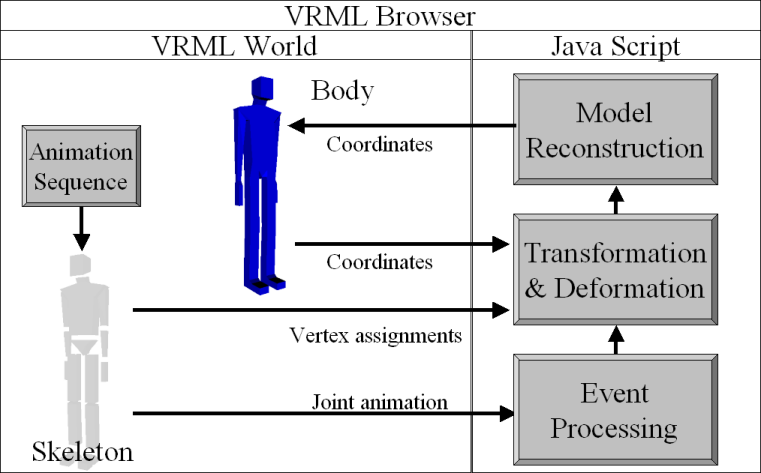
\includegraphics[width=10cm]{../images/systemdiagram2}
\caption{\label{fig:overview} System Overview}
\end{center}
\end{figure}

Animation is applied to the H-Anim skeleton as usual, but is also passed on to the {\bf Script}, which uses the joint rotations to deform the coordinates from each segment each frame. These coordinates are then placed into an {\bf IndexedFaceSet} which already contains the topology of the mesh, along with texture information, giving a complete model.

\section{\label{sec:segments}Segments}
If we consider the {\bf Segment} node as defined in the H-Anim 1.1 specification\cite{HANIM:1.1} (shown in figure \ref{fig:segmentproto}), we can see that part of the architecture for deformable meshes is already in place, with the {\it coord} field. To quote the specification:

\begin{quote}
For Segments that have deformable meshes, the coord field should contain a Coordinate node that is USEd in the IndexedFaceSet for the Segment. The Coordinate node should be given the same name DEF name as the Segment, but with "\_coords" appended (e.g. "skull\_coords").
\end{quote}

\begin{figure}[th]
\scriptsize
\begin{verbatim}
PROTO Segment [
 field        SFVec3f    bboxCenter       0 0 0
 field        SFVec3f    bboxSize         -1 -1 -1
 exposedField SFVec3f    centerOfMass     0 0 0
 exposedField MFNode     children         []
 exposedField SFNode     coord            NULL
 exposedField MFNode     displacers       []
 exposedField SFFloat    mass             0
 exposedField MFFloat    momentsOfInertia [ 0 0 0 0 0 0 0 0 0 ]
 exposedField SFString   name             ""
 eventIn      MFNode     addChildren
 eventIn      MFNode     removeChildren
]
\end{verbatim}
\caption{\label{fig:segmentproto} The Segment prototype}
\end{figure}

Our system adheres to the original intent of the group in this case, by storing the coordinates associated with a particular segment inside a {\bf Coordinate} node inside the {\it coord} field of that segment. This {\bf Coordinate} node is not USEd in an {\bf IndexedFaceSet} for the segment as suggested, but such an arrangement is certainly possible. The Coordinate nodes are also named in accordance with the groups recommendations.

\section{\label{sec:humanoid}The extended Humanoid node}
In order to display our deformable models, which are a single mesh, we will need somewhere to store the deformed vertex positions, along with the texture and colour information that make up the final model. This need will be filled by creating a new node type, which will be explained below. This new node is contained inside the new {\it meshBody} field which is part of the {\bf Humanoid} node. The extended {\bf Humanoid} node is shown in figure \ref{fig:humanoidproto}.

\begin{figure}[th]
\scriptsize
\begin{verbatim}
PROTO Humanoid [
 exposedField SFString   name             ""
 exposedField MFString   info             []
 exposedField SFString   version          "1.1"
 exposedField MFNode     joints           []
 exposedField MFNode     segments         []
 exposedField MFNode     sites            []
 exposedField MFNode     viewpoints       []
 exposedField MFNode     humanoidBody     []
 exposedField SFNode     meshBody         NULL
 exposedField SFVec3f    center           0 0 0
 exposedField SFRotation rotation         0 0 1 0
 exposedField SFVec3f    scale            1 1 1
 exposedField SFRotation scaleOrientation 0 0 1 0
 exposedField SFVec3f    translation      0 0 0
]
{
  Transform {
    center IS center
    rotation IS rotation
    scale IS scale
    scaleOrientation IS scaleOrientation
    translation IS translation
    children [
      Group {
        children IS viewpoints
      }
      Group {
        children IS humanoidBody
      }
      Group {
        children IS meshBody
      }
    ]
  }
}
\end{verbatim}
\caption{\label{fig:humanoidproto} The extended Humanoid prototype}
\end{figure}

The node inside the {\it meshBody} field is contained inside a {\bf Group} at the same level of the transformation hierarchy as the HumanoidRoot joint. This is desirable, as we want the deformable body to be affected by transformations of the complete body, but not by transformations of the joint hierarchy, as these involve deforming the body shape itself.

\section{\label{sec:meshbody}The MeshBody node}
A new node type is required which will contain the topology of the final model, along with any texture and colour information. This is the {\bf MeshBody} node, and is contained within the {\it meshBody} field of the {\bf Humanoid} node. This is implemented as a new PROTO, which is shown in figures \ref{fig:meshbodyproto} and \ref{fig:meshbodyprotoimpl}.

\begin{figure}[th]
\scriptsize
\begin{verbatim}
PROTO MeshBody [
 exposedField SFString   name             ""
 exposedField MFString   info             []
 exposedField SFNode     appearance       NULL
 exposedField SFNode     color            NULL
 exposedField SFNode     normal           NULL
 exposedField SFNode     texCoord         NULL     
 field        SFBool     ccw              TRUE
 field        MFInt32    colorIndex       []
 field        SFBool     colorPerVertex	  TRUE
 field        SFBool     convex           TRUE
 field        MFInt32    coordIndex       []
 field        SFFloat    creaseAngle      0
 field        MFInt32    normalIndex      []
 field        SFBool     normalPerVertex  TRUE
 field        SFBool     solid            TRUE
 field        MFInt32    texCoordIndex    []
 field        SFBool     mustEvaluate     FALSE
 field        SFNode     humanoid         NULL
 field        MFString   url              []
 eventIn      SFVec3f    HumanoidRoot_translation_changed
 eventIn      SFRotation HumanoidRoot_rotation_changed
 eventIn      SFRotation l_hip_rotation_changed
 eventIn      SFRotation l_knee_rotation_changed
 eventIn      SFRotation l_ankle_rotation_changed
 eventIn      SFRotation l_midtarsal_rotation_changed
 ...likewise for each joint...
]
\end{verbatim}
\caption{\label{fig:meshbodyproto} The MeshBody prototype}
\end{figure}

\begin{figure}[th]
\scriptsize
\begin{verbatim}
{
  Group {
    children [
      Shape {
        appearance IS appearance
        geometry IndexedFaceSet {
          color IS color
          normal IS normal
          texCoord IS texCoord
          ccw IS ccw
          colorIndex IS colorIndex
          colorPerVertex IS colorPerVertex
          convex IS convex
          coordIndex IS coordIndex
          coord DEF BODYCOORDS Coordinate {}
          creaseAngle IS creaseAngle
          normalIndex IS normalIndex
          normalPerVertex IS normalPerVertex
          solid IS solid
          texCoordIndex IS texCoordIndex
        }
      }
      DEF SEAMLESSBODY Script {
        url IS url
        directOutput TRUE
        mustEvaluate IS mustEvaluate
        field SFNode humanoid IS humanoid
        field SFNode bodyCoords USE BODYCOORDS
        eventIn SFVec3f    translation  IS  HumanoidRoot_translation_changed
        eventIn SFRotation HumanoidRoot IS  HumanoidRoot_rotation_changed
        eventIn SFRotation l_hip        IS  l_hip_rotation_changed
        eventIn SFRotation l_knee       IS  l_knee_rotation_changed
        eventIn SFRotation l_ankle      IS  l_ankle_rotation_changed
        eventIn SFRotation l_midtarsal  IS  l_midtarsal_rotation_changed
        ...likewise for each joint...
      }
    ]
  }
}
\end{verbatim}
\caption{\label{fig:meshbodyprotoimpl} Implementation of the MeshBody prototype}
\end{figure}

The node is basically an {\bf IndexedFaceSet} and {\bf Script}. The IFS will contain the texture, colour and topology for a complete model, and the Script will generate the coordinates for the IFS each frame as the model moves. The Script can place the coordinates directly into the Coordinate node of the IFS by using it's {\it bodyCoords} field, recreating a complete model each frame.

The {\it humanoid} field should USE the main {\bf Humanoid} node, so that the script can access it's fields and children.

There are also a set of eventIns for the transformations of the joint hierarchy, which will be used by the script. These need to be ROUTEd from the joint hierarchy itself or directly from the animation source. There is also a {\it deform} field, which is specific to our deformation engine. This is used to choose the style of deformation that will be performed by the deformation engine. This should not appear in the final specification, and should be removed or replaced with something more independant of the deformation engine.

There are many improvements that can be made to the layout and operation of this node. See section \ref{sec:improvements} for more details.

\section{\label{sec:deformation}The deformation engine}
The implementation of the deformation engine is left up to the content creator. One implementation has already been developed at the University of Surrey, and is used to drive a number of models, which are available at http://www.ee.surrey.ac.uk/Personal/R.Smith/hanim/seamless/.

The script can be implemented in any available language, using any animation method. The only requirements are that the script should produce a new list of coordinates every frame, and place them in the Coordinate node of the IFS in the MeshBody. This vertex list should be ordered in the following fashion. Starting at the beginning of the {\it segments} field in the {\bf Humanoid}, the new vertices from the first segment should be output, followed by the new vertices from the second, and so on until all vertices have been output.

\section{\label{sec:modeling}Modeling requirements}
This proposal requires no particular geometric arrangment of vertices in the model, or any special parameterisations. All that is required is a normal static model of a human, as would be generated the VRML export of any 3D modeling pacakge. The vertex list of this model is split into sections and placed in the Segments, and all other model information is stored in the MeshBody.

However, the model will be recreated by joining the vertices in the segments in order of the appearance of the segments in the {\it segments} field in the {\bf Humanoid}. So, the ordering of the vertices in the original model is important if the final model is to make sense when it is reconstructed.

\section{\label{sec:improvements}Suggetions \& Improvements}
This section presents some brief ideas for improvements to the proposal that we have come up with during the course of implementation.

\begin{itemize}
\item If the segments do not contain actual coordinates, but instead contain offsets into a single vertex list, then the model needs no special ordering at all, making it very simple to model. This also has the advantage that vertices can be associated with more than one segment, which may be desirable in the future when more computing power is available for more complex deformation schemes.
\item The {\bf Script} could look up new joint positions by traversing the joint hierarchy, instead of having to have a large number of extra ROUTEs.
\item {\it Suggested by Bernie Roehl:} The {\bf MeshBody} node should also have an eventIn (which would be IS'd to the {\bf Script}) that allows applications to write to the entire coordinate array.  This will allow us to easily support the sort of animation that's done in many computer games, where each sequence is essentially just a {\bf CoordinateInterpolator} that replaces all the vertices in the body.
\end{itemize}

\bibliographystyle{abbrv}
\bibliography{../bib/papers,../bib/r.smith}

\end{document}
